\qquad La teoría de Heath, Jarrow y Morton (HJM) provee un marco general para modelar las tasas de interés. En su enfoque, se describe la dinámica de la curva de tasas de interés de manera estocástica, considerando que las tasas futuras forman un proceso multivariado sujeto a incertidumbre. Esta teoría sirve como base conceptual para modelos de tasas de interés, incluido el modelo de Ho–Lee.

\qquad La idea central dentro de la teoría HJM es modelar la tasa libre de riesgo (o tasa cero cupón) como un proceso de Itô que satisface la ecuación
\begin{equation}
    dr(t) = \mu(r,t)\,dt + \sigma(r,t)\,dW(t),
\end{equation}
donde $\mu$ es el \emph{drift} del modelo, $\sigma$ es la volatilidad instantánea de la tasa $r$ y $W$ es un movimiento browniano estándar.

\subsection{El modelo de Ho--Lee}

\qquad El modelo de Ho--Lee es un caso particular del marco anterior, en el que las tasas de interés a corto plazo se modelan como un proceso estocástico lineal:
\begin{equation}
    dr(t) = \theta(t)\,dt + \sigma\,dW(t),
\end{equation}
donde $r(t)$ es la tasa instantánea en el tiempo $t$, $\theta(t)$ es un término determinista que asegura el ajuste a la curva de tasas inicial, $\sigma$ es la volatilidad constante y $W(t)$ es un movimiento browniano estándar.

\qquad Decir que un mercado es libre de arbitraje significa que no existen oportunidades de obtener una ganancia con inversión neta nula. Bajo este concepto, el modelo de Ho--Lee es libre de arbitraje.

\subsection{Versión discreta del modelo}

\qquad En su versión discreta, el modelo se escribe como
\begin{equation}
    r_{t+\Delta t} = r_t + \theta_t\,\Delta t + \sigma \sqrt{\Delta t}\,\varepsilon_t,
\end{equation}
donde $\varepsilon_t \sim \mathcal{N}(0,1)$ es una variable aleatoria normal estándar (proviene de discretizar el movimiento browniano) y $\Delta t$ es el tamaño del paso temporal. Esta formulación es especialmente útil para simulaciones numéricas y para la valoración de instrumentos financieros en árboles binomiales, como se hizo en este trabajo.

\qquad Con la modelación anterior para $r_{t+\Delta t}$, se generan distintas posibilidades para la tasa en cada paso de tiempo, dando origen a árboles como el de la figura \ref{fig:arbolHL}.

\begin{figure}[h]
    \centering
    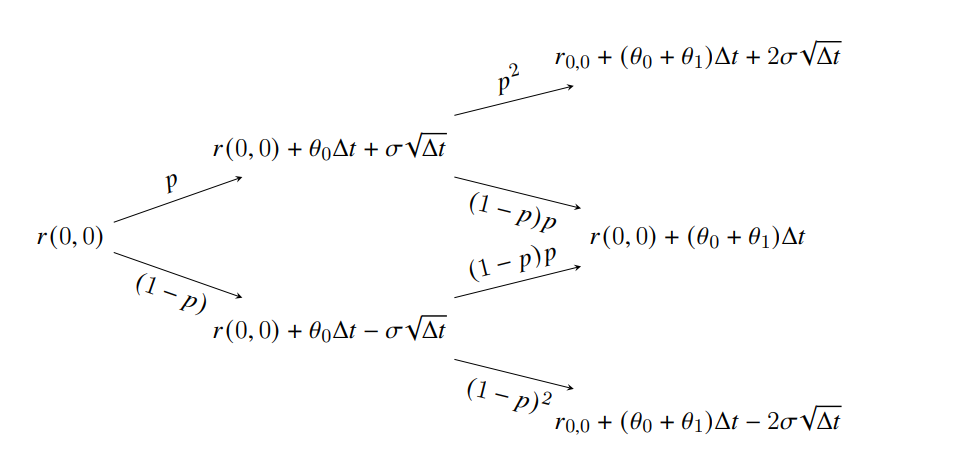
\includegraphics[scale=0.5]{images/grafico_Ho_Lee.png}
    \caption{Ejemplo de árbol generado por el modelo de Ho--Lee.}
    \label{fig:arbolHL}
\end{figure}
\paragraph{Pros de la versión discreta:}
\begin{itemize}
    \item Facilita la implementación computacional, especialmente para bonos y derivados, además de reducir los tiempos de cómputo.
    \item Permite integrar datos de mercado de manera directa y generar árboles de tasas consistentes con la curva inicial.
\end{itemize}

\qquad El uso de este árbol para la valoración de créditos corporativos consiste en calcular el valor del crédito en cada nodo del árbol a partir de las trayectorias de la tasa de interés. El siguiente paso es traer estos valores a presente usando la tasa vigente hasta la fecha del nodo. Luego se estima la esperanza del valor del crédito como el promedio de los valores presentes del crédito en todos los nodos.

\qquad Con base en el procedimiento anterior, se puede ajustar la tasa de interés que se ofrece al cliente en el tiempo inicial para que el retorno promedio de la institución financiera sea el deseado. Esta herramienta permite considerar créditos a distintos plazos, cortando el árbol cuando $t+n\Delta t$ (con $n$ el número de pasos temporales) alcanza el plazo de interés, y a partir de ello realizar los cálculos.
